\section{Hell}

\begin{center}
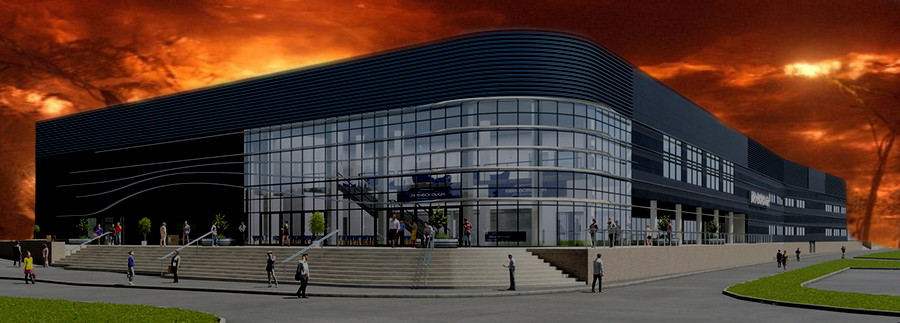
\includegraphics[width=80mm]{./content/img/hellBuilding.jpg}
\begin{figure}[h]
\end{figure}
\end{center}

One of the dimensions of the afterlife. It's hot.

\section{Main Land}

\begin{center}
%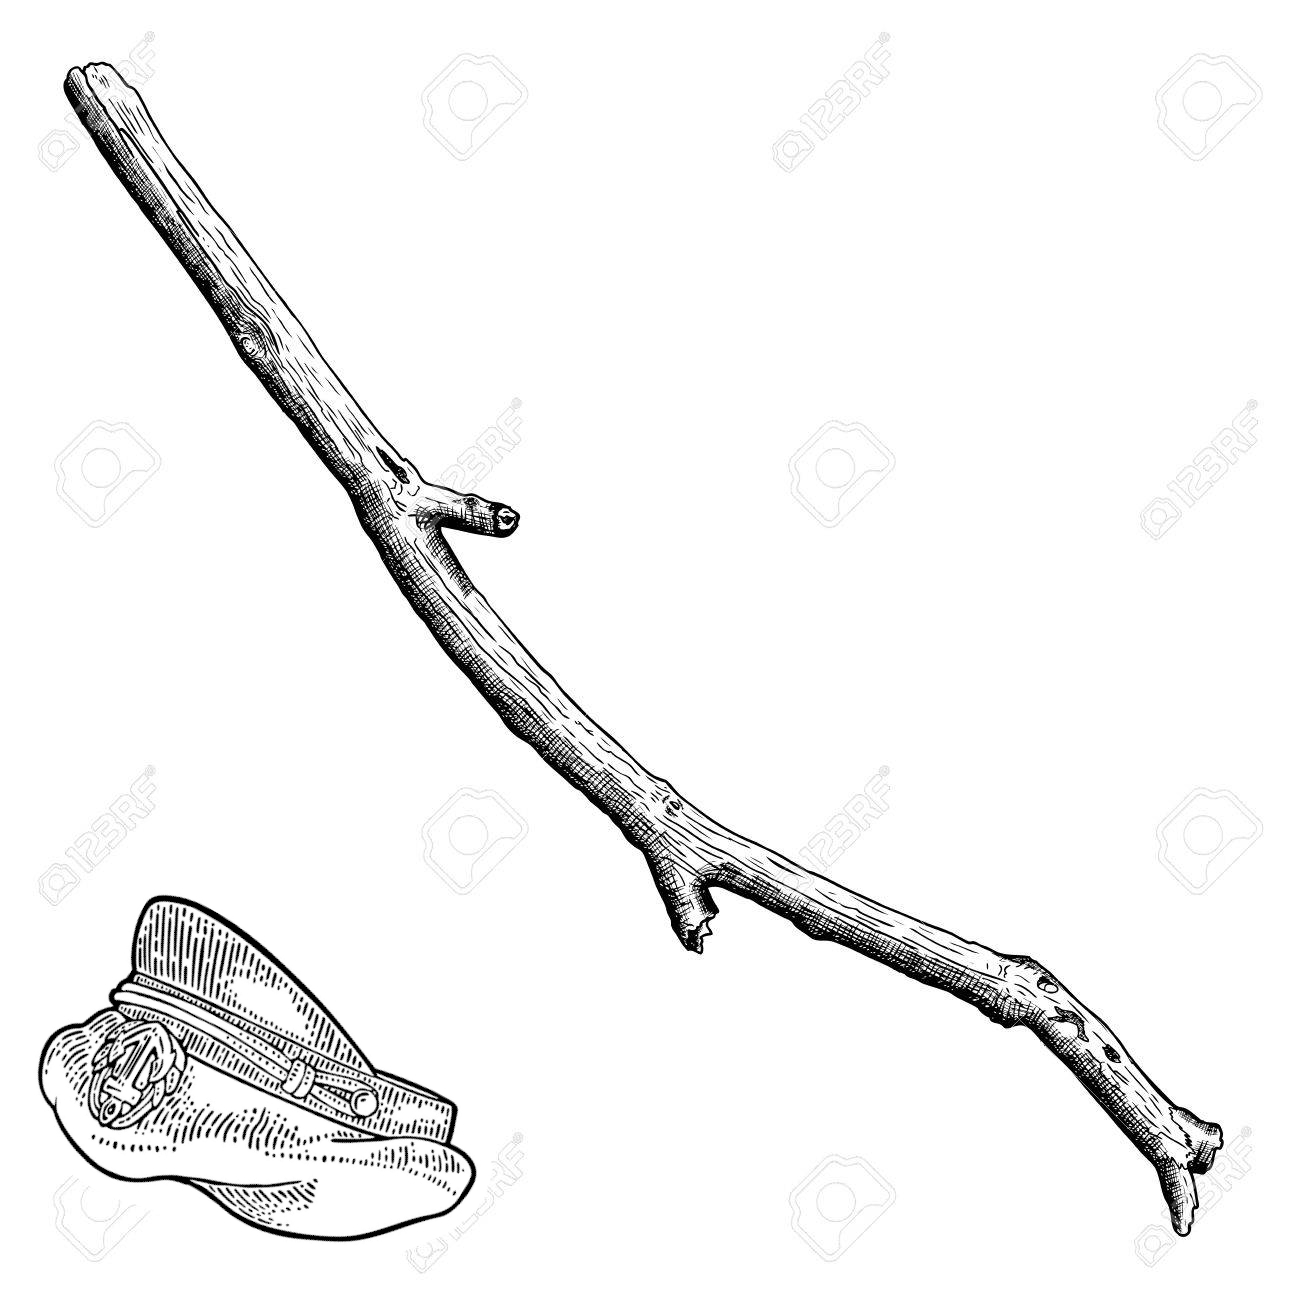
\includegraphics[width=80mm]{./content/img/mainLand/xxx.png}
%\begin{figure}[h]
%\end{figure}
\end{center}


\subsection*{Hope's Rest} 

\vspace{5mm}

\begin{center}
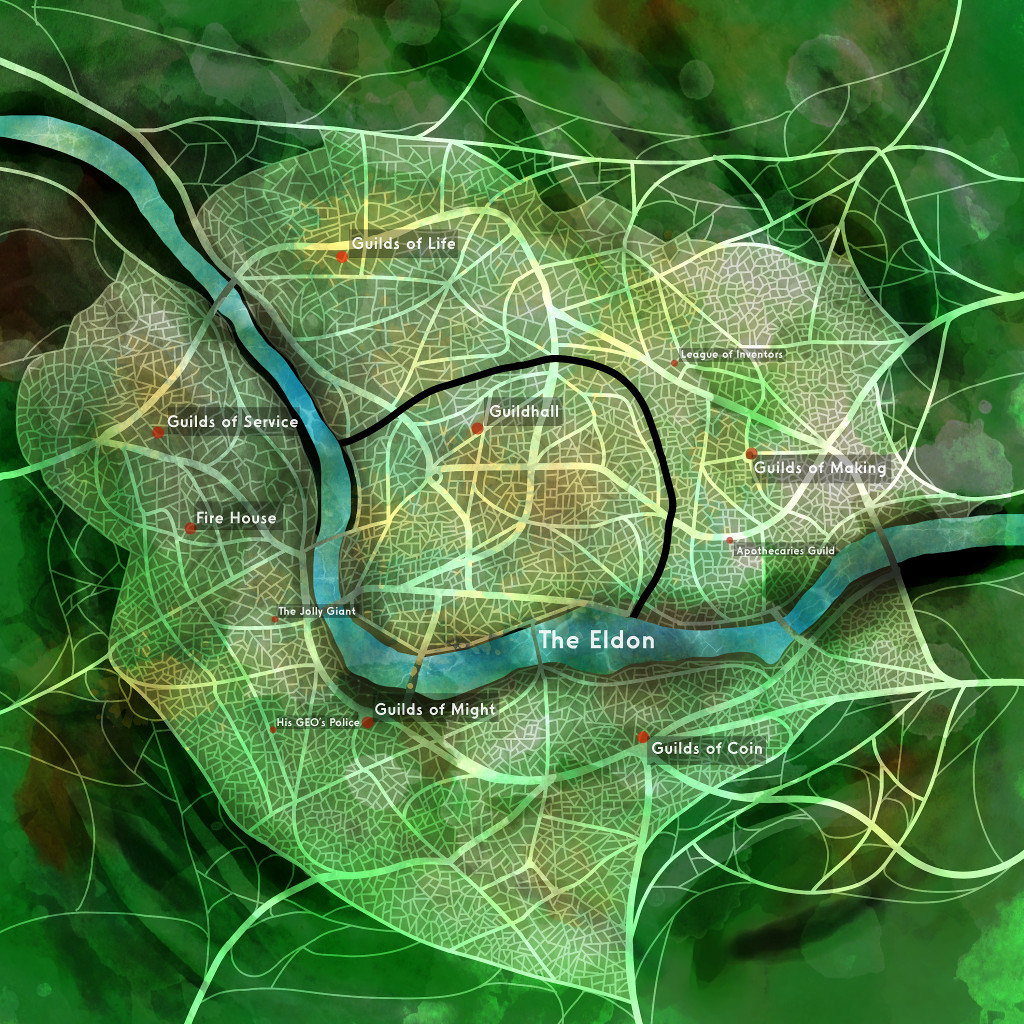
\includegraphics[width=80mm]{./content/img/hopesRest.png}
\begin{figure}[h]
\end{figure}
\end{center}

\noindent 

The biggest city in Velterra.

Central mecca of trading for the region controlled by the church. Very multi-cultural.

City is broken up into its Guilds from the old families of the city.

Each family selects a board that selects a GEO Guild Executive Officer that rules the area.

Parchet green (half elf) male quite stern, and ruthless. All who stood against him in elections have vanished.

The five families have guilds underneath them,

    Life = taverns, gambling,
    Might = Archers, mercenaries, masters elite unit, the hunt (bounty hunters for beasts)
    Coin = traders, stores, market, and mint
    Service = cleaners, valets, plumbers, Jennies (semi official), Theives Guild, Assasins Guild
    Making = carpenters, builders, blacksmiths, clothiers etc

River Eldon flows through the middle. The areas have power over the sections of the town, but also the guild members who live outside of the guild area.

Politics area is around the Guild Hall.

Bertrands stand is the last defensive wall.

The Petite Ferret is owned and run by Horatio BrambleThrust

The Book Burners is the location of their old library, staffed by good old Archibald

\smallskip

\subsubsection*{The Book Burner's Headquarters} 

\vspace{5mm}

\begin{center}
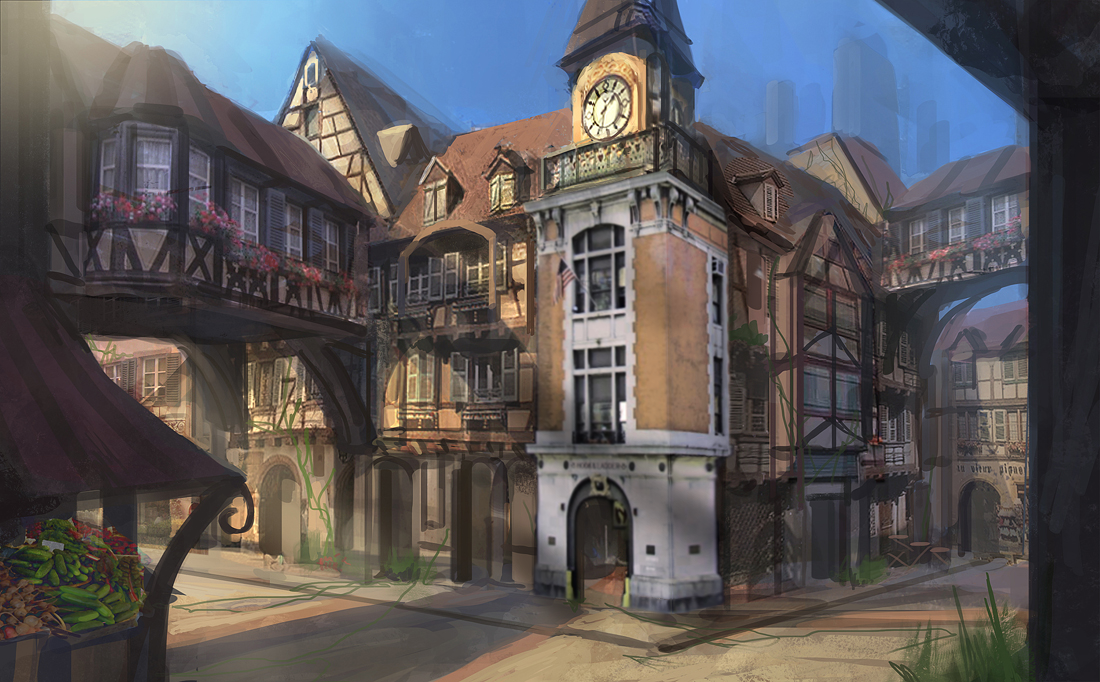
\includegraphics[width=80mm]{./content/img/bookBurnerBase.png}
\begin{figure}[h]
\end{figure}
\end{center}

\noindent 

Text

\smallskip

\subsection*{Vathos Boundary} 

A small settlement on the edge of the civilized world. The last stop before the southern wilderness.
Buildings

    Pub 1 Copper Flagon
    Pub 2 "Titty bar"
    Black smith
    Pastor Dunkhills Church
    City Guard House
    Jewellers
    Stable

CountrySide

    Dutty Hoes Camp
    RWA cave hideout
    Forest of Big Pig


\smallskip

\subsection*{Tom'ardy Mountains} 

Home to an exclusive and reclusive enclave of high-status Dwarven families. Each dynasty resides in their own private mountain. It can take days just to say hello to your neighbours... not that anyone does.

\smallskip

\subsection*{Temple of Unthala} 

\smallskip

\subsection*{Riverfall} 

\vspace{5mm}

\begin{center}
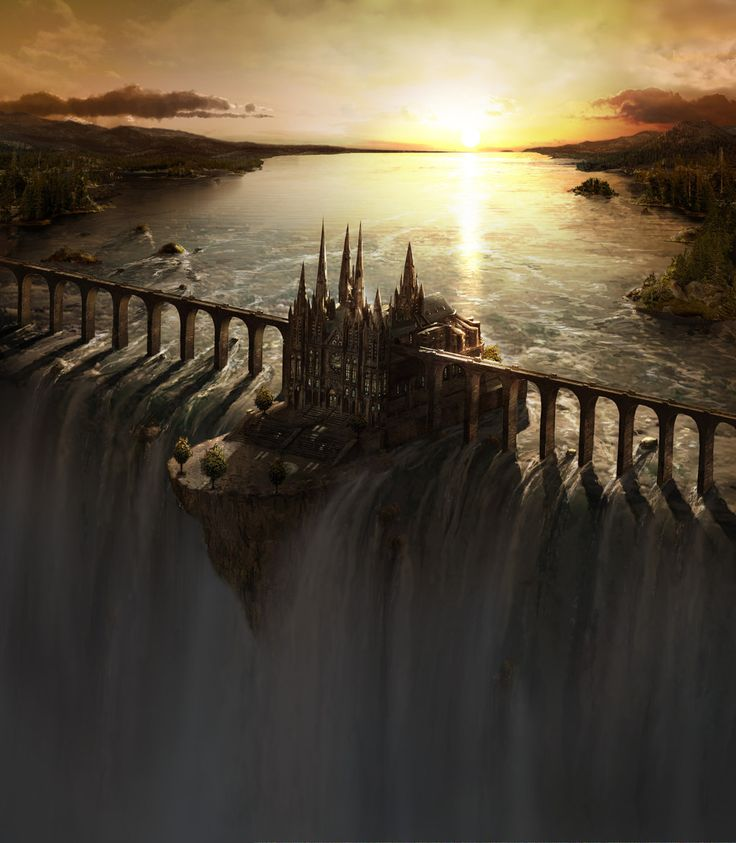
\includegraphics[width=80mm]{./content/img/riverfall.png}
\begin{figure}[h]
\end{figure}
\end{center}

\noindent 

More is known about RiversFall, except that it has a beautiful set of rivers and waterfalls.

Its is a fair to middling size of town.

Had four pubs (Sad Crusader, Club and Cask, Open Flask, Minstrels) , once of which unfortunately and mysteriously burnt down.
It also has a very expensive black smith
There is also a Tower of Emoticon, that houses a whole load of secret stuff in a vault and a lovely collection of non religious but church safe books

A new edition to the town is a nicely sized ditch on the outskirts

\begin{DndSidebar}{Fallen Twin}
 dfhgsfdghfsgh
\end{DndSidebar}

\smallskip

\subsection*{The Seven's Spire} 

\vspace{5mm}

\begin{center}
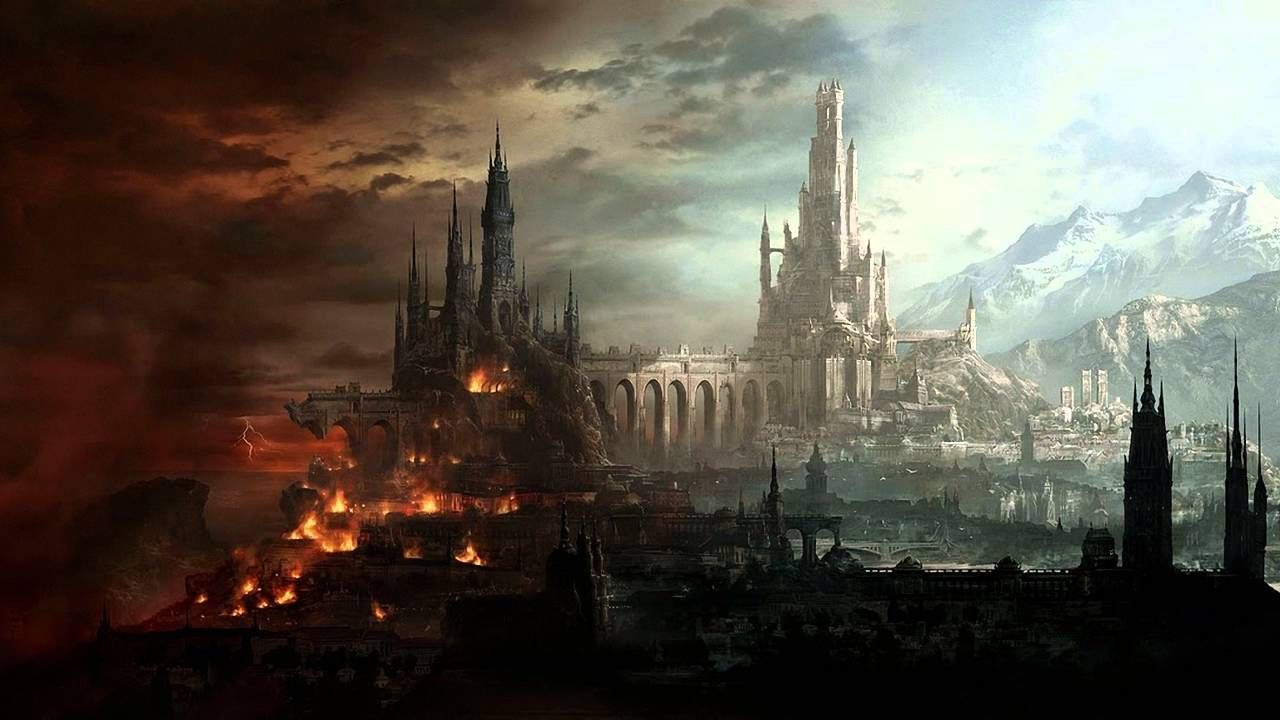
\includegraphics[width=80mm]{./content/img/7spire.jpg}
\begin{figure}[h]
\end{figure}
\end{center}

\noindent 

\subsection*{Tower of Imota Kan} 

\smallskip

\subsection*{Largosk} 

\vspace{5mm}

\begin{center}
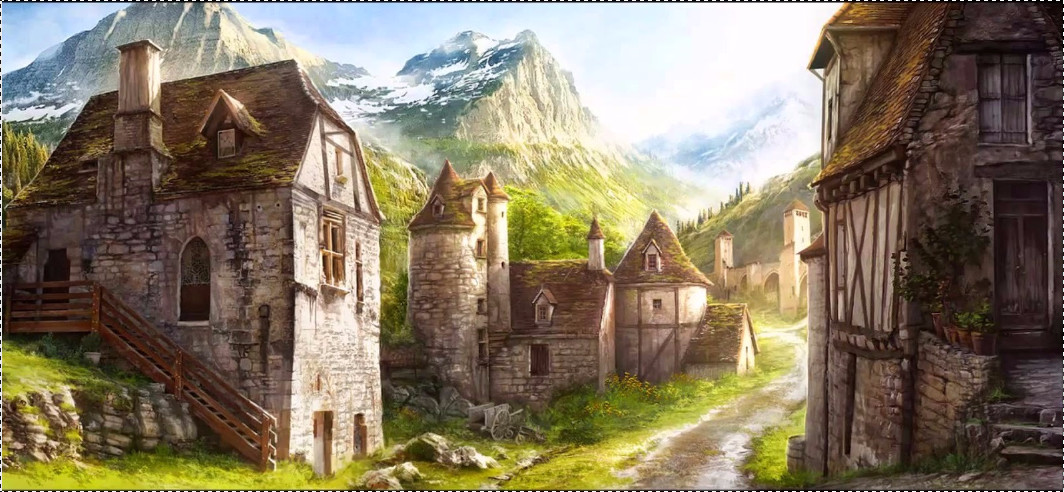
\includegraphics[width=80mm]{./content/img/largosk.png}
\begin{figure}[h]
\end{figure}
\end{center}

\noindent 

Nice sleepy town that takes its children through a trial at the age of 5. We arrived here while on the Lamb from a scary inquisitor. Over the mountains is SevenSpires!

This is where we first encountered the Spanish inquisition. While saving a small boy from a horrid coming of age ceremony, we were ambushed by the Inquisition who wanted to take the child as their own. Not cool. Kyros later tried to blame us for the mess, but is now more neutrally disposed to us. That is until she finds out about the dirty lemon whores who stole a poor couples only lemons, to have a bake sale! 

\subsection*{The Great Expanse} 

A land of empty desert, people get lost often within its borders and the area is plagued by "bandits" called spansers. This anti-church group preys upon the Great Expanses travelers. 

\smallskip

\subsection*{Port Averdale} 

One of the major ports on the main continent. This port was full of colourful people and shady goings on. What it really needed was a show from a circus troupe, but we failed them. They do have a lovely square made up of two triangles that hosts all kinds of cultural events.

It also had a lovely customs expo, that was mysteriously burned down.

\smallskip



\section{Nanduan} 

Nanduan is a large kingdom on the North-Eastern coast of the continent of Erassa. The capital city is located on the banks of a tidal river estuary, and maritime trade makes up a significant portion of the economy.

Nanduan does not trade significantly with Velarian cities, but has some relations with the elven city of A'kul'theok. There is limited migration from Nanduan to Church-controlled cities, and so not much is known about this land by commoners in these areas. Traders and travellers may have some patchy information. It is known that relations between Nanduan and Masuda, to the south, are strained, at best.
Known Inhabitants

    The Hearthrust Dynasty - A large, wealthy and prominent noble family. They recognise the danger of the isolation their social class gives them, and therefore the children of each generation are sent out into the world for a few years at the age of 18 to experience what life is like for the people below them. Some run small businesses, some join religious orders, but most use the opportunity to become adventurers or travelers. As most marriages within the family are arranged during the teenage years, some of the Hearthrust children are already betrothed by the time they begin their travels. In this case, the face of the Hearthrust daughters are covered, to save the world the pain of seeing, but not being able to attain, such beauty. Hearthrust girls are renowned in Naduan as being exceptionally beautiful.

    They are also seen as beautiful in their own country of Nanduan.

    An Unnamed Shipping Magnate - Known to be betrothed to Lady Otoria Hearthrust.

Flora and Fauna

    Sand Dagger - Dangerous and sneaky creatures known to hide underneath and behind things.

    Balloon Cow - Like cows, but inflatable.


\smallskip


\section{South Africa}

\vspace{5mm}

\begin{center}
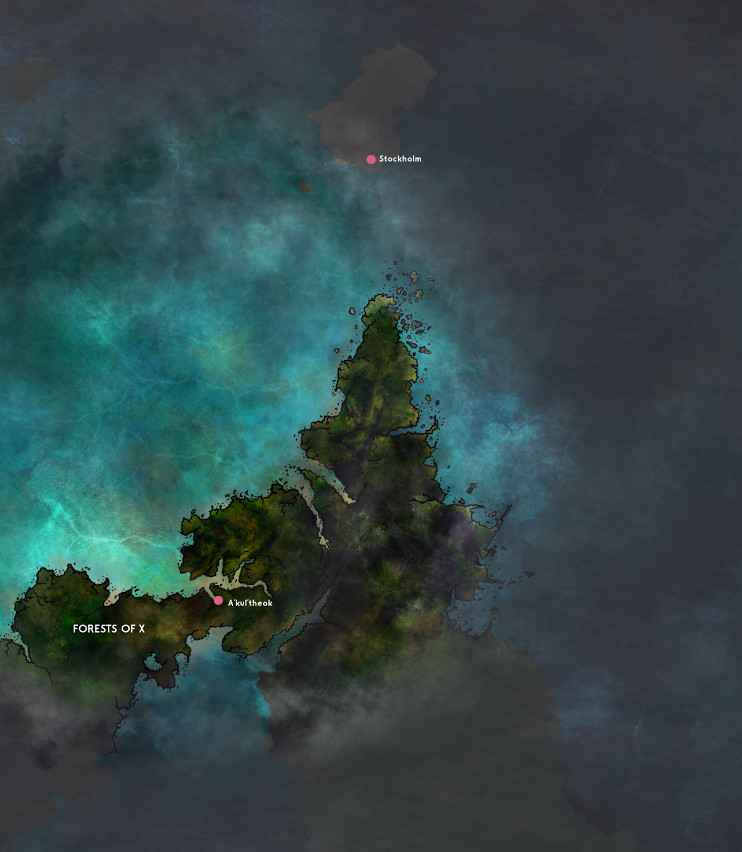
\includegraphics[width=80mm]{./content/img/southAfrica.png}
\begin{figure}[h]
\end{figure}
\end{center}

\noindent 

\subsection*{Akultheok} 

Akultheok is the main port on the continent of South Africa, it was relatively friendly and very much like a Caribbean beach resort complete with great cocktails. However the surrounding jungles are as dangerous as the come. 

\smallskip

\subsection*{Jungles} 

Super dangerous Jungles, full off tribes, trebuchets, and Cannibal Tikki Tucks. Somewhere in here is the Rubriks Cube that we so desire

\smallskip


\bigskip

%\begin{DndSidebar}[float=!b]{Behold the DndSidebar!}
 %dfhgsfdghfsgh
%\end{DndSidebar}

\clearpage
